% Options for packages loaded elsewhere
\PassOptionsToPackage{unicode}{hyperref}
\PassOptionsToPackage{hyphens}{url}
%
\documentclass[
]{article}
\usepackage{amsmath,amssymb}
\usepackage{iftex}
\ifPDFTeX
  \usepackage[T1]{fontenc}
  \usepackage[utf8]{inputenc}
  \usepackage{textcomp} % provide euro and other symbols
\else % if luatex or xetex
  \usepackage{unicode-math} % this also loads fontspec
  \defaultfontfeatures{Scale=MatchLowercase}
  \defaultfontfeatures[\rmfamily]{Ligatures=TeX,Scale=1}
\fi
\usepackage{lmodern}
\ifPDFTeX\else
  % xetex/luatex font selection
\fi
% Use upquote if available, for straight quotes in verbatim environments
\IfFileExists{upquote.sty}{\usepackage{upquote}}{}
\IfFileExists{microtype.sty}{% use microtype if available
  \usepackage[]{microtype}
  \UseMicrotypeSet[protrusion]{basicmath} % disable protrusion for tt fonts
}{}
\makeatletter
\@ifundefined{KOMAClassName}{% if non-KOMA class
  \IfFileExists{parskip.sty}{%
    \usepackage{parskip}
  }{% else
    \setlength{\parindent}{0pt}
    \setlength{\parskip}{6pt plus 2pt minus 1pt}}
}{% if KOMA class
  \KOMAoptions{parskip=half}}
\makeatother
\usepackage{xcolor}
\usepackage[margin=1in]{geometry}
\usepackage{color}
\usepackage{fancyvrb}
\newcommand{\VerbBar}{|}
\newcommand{\VERB}{\Verb[commandchars=\\\{\}]}
\DefineVerbatimEnvironment{Highlighting}{Verbatim}{commandchars=\\\{\}}
% Add ',fontsize=\small' for more characters per line
\usepackage{framed}
\definecolor{shadecolor}{RGB}{248,248,248}
\newenvironment{Shaded}{\begin{snugshade}}{\end{snugshade}}
\newcommand{\AlertTok}[1]{\textcolor[rgb]{0.94,0.16,0.16}{#1}}
\newcommand{\AnnotationTok}[1]{\textcolor[rgb]{0.56,0.35,0.01}{\textbf{\textit{#1}}}}
\newcommand{\AttributeTok}[1]{\textcolor[rgb]{0.13,0.29,0.53}{#1}}
\newcommand{\BaseNTok}[1]{\textcolor[rgb]{0.00,0.00,0.81}{#1}}
\newcommand{\BuiltInTok}[1]{#1}
\newcommand{\CharTok}[1]{\textcolor[rgb]{0.31,0.60,0.02}{#1}}
\newcommand{\CommentTok}[1]{\textcolor[rgb]{0.56,0.35,0.01}{\textit{#1}}}
\newcommand{\CommentVarTok}[1]{\textcolor[rgb]{0.56,0.35,0.01}{\textbf{\textit{#1}}}}
\newcommand{\ConstantTok}[1]{\textcolor[rgb]{0.56,0.35,0.01}{#1}}
\newcommand{\ControlFlowTok}[1]{\textcolor[rgb]{0.13,0.29,0.53}{\textbf{#1}}}
\newcommand{\DataTypeTok}[1]{\textcolor[rgb]{0.13,0.29,0.53}{#1}}
\newcommand{\DecValTok}[1]{\textcolor[rgb]{0.00,0.00,0.81}{#1}}
\newcommand{\DocumentationTok}[1]{\textcolor[rgb]{0.56,0.35,0.01}{\textbf{\textit{#1}}}}
\newcommand{\ErrorTok}[1]{\textcolor[rgb]{0.64,0.00,0.00}{\textbf{#1}}}
\newcommand{\ExtensionTok}[1]{#1}
\newcommand{\FloatTok}[1]{\textcolor[rgb]{0.00,0.00,0.81}{#1}}
\newcommand{\FunctionTok}[1]{\textcolor[rgb]{0.13,0.29,0.53}{\textbf{#1}}}
\newcommand{\ImportTok}[1]{#1}
\newcommand{\InformationTok}[1]{\textcolor[rgb]{0.56,0.35,0.01}{\textbf{\textit{#1}}}}
\newcommand{\KeywordTok}[1]{\textcolor[rgb]{0.13,0.29,0.53}{\textbf{#1}}}
\newcommand{\NormalTok}[1]{#1}
\newcommand{\OperatorTok}[1]{\textcolor[rgb]{0.81,0.36,0.00}{\textbf{#1}}}
\newcommand{\OtherTok}[1]{\textcolor[rgb]{0.56,0.35,0.01}{#1}}
\newcommand{\PreprocessorTok}[1]{\textcolor[rgb]{0.56,0.35,0.01}{\textit{#1}}}
\newcommand{\RegionMarkerTok}[1]{#1}
\newcommand{\SpecialCharTok}[1]{\textcolor[rgb]{0.81,0.36,0.00}{\textbf{#1}}}
\newcommand{\SpecialStringTok}[1]{\textcolor[rgb]{0.31,0.60,0.02}{#1}}
\newcommand{\StringTok}[1]{\textcolor[rgb]{0.31,0.60,0.02}{#1}}
\newcommand{\VariableTok}[1]{\textcolor[rgb]{0.00,0.00,0.00}{#1}}
\newcommand{\VerbatimStringTok}[1]{\textcolor[rgb]{0.31,0.60,0.02}{#1}}
\newcommand{\WarningTok}[1]{\textcolor[rgb]{0.56,0.35,0.01}{\textbf{\textit{#1}}}}
\usepackage{graphicx}
\makeatletter
\def\maxwidth{\ifdim\Gin@nat@width>\linewidth\linewidth\else\Gin@nat@width\fi}
\def\maxheight{\ifdim\Gin@nat@height>\textheight\textheight\else\Gin@nat@height\fi}
\makeatother
% Scale images if necessary, so that they will not overflow the page
% margins by default, and it is still possible to overwrite the defaults
% using explicit options in \includegraphics[width, height, ...]{}
\setkeys{Gin}{width=\maxwidth,height=\maxheight,keepaspectratio}
% Set default figure placement to htbp
\makeatletter
\def\fps@figure{htbp}
\makeatother
\setlength{\emergencystretch}{3em} % prevent overfull lines
\providecommand{\tightlist}{%
  \setlength{\itemsep}{0pt}\setlength{\parskip}{0pt}}
\setcounter{secnumdepth}{5}
\ifLuaTeX
  \usepackage{selnolig}  % disable illegal ligatures
\fi
\IfFileExists{bookmark.sty}{\usepackage{bookmark}}{\usepackage{hyperref}}
\IfFileExists{xurl.sty}{\usepackage{xurl}}{} % add URL line breaks if available
\urlstyle{same}
\hypersetup{
  pdftitle={A Brief Intro to R with R Markdown},
  pdfauthor={Cheng Peng},
  hidelinks,
  pdfcreator={LaTeX via pandoc}}

\title{A Brief Intro to R with R Markdown}
\author{Cheng Peng}
\date{STA 490 Statistics Capstone}

\begin{document}
\maketitle

{
\setcounter{tocdepth}{4}
\tableofcontents
}
\hypertarget{introduction}{%
\subsubsection{Introduction}\label{introduction}}

This brief note will introduce the basics of Rstudio, R Markdown, and R.

\begin{itemize}
\item
  \textbf{RStudio} is an integrated development environment (IDE) for R.
  It includes a console, syntax-highlighting editor that supports direct
  code execution, as well as tools for plotting, history, debugging and
  work space management.
\item
  \textbf{R Markdown} is a file format for making dynamic documents with
  R. An R Markdown document is written in markdown (an easy-to-write
  plain text format) and contains chunks of embedded R code and the
  output generated from the R code. This note is written in R Markdown.
  This is also a tutorial showing how to use R Markdown to write an R
  Markdown report. -- RStudio documentation.
\item
  \textbf{R} is a language and environment for statistical computing and
  graphics. It is a GNU project which is similar to the S language and
  environment which was developed at Bell Laboratories (formerly AT\&T,
  now Lucent Technologies) by John Chambers and colleagues. R can be
  considered as a different implementation of S. There are some
  important differences, but much code written for S runs unaltered
  under R.
\end{itemize}

\hypertarget{rstudio-gui}{%
\subsubsection{RStudio GUI}\label{rstudio-gui}}

The RStudio interface consists of several windows. I insert an image of
a regular RStudio GUI.

\begin{figure}

{\centering 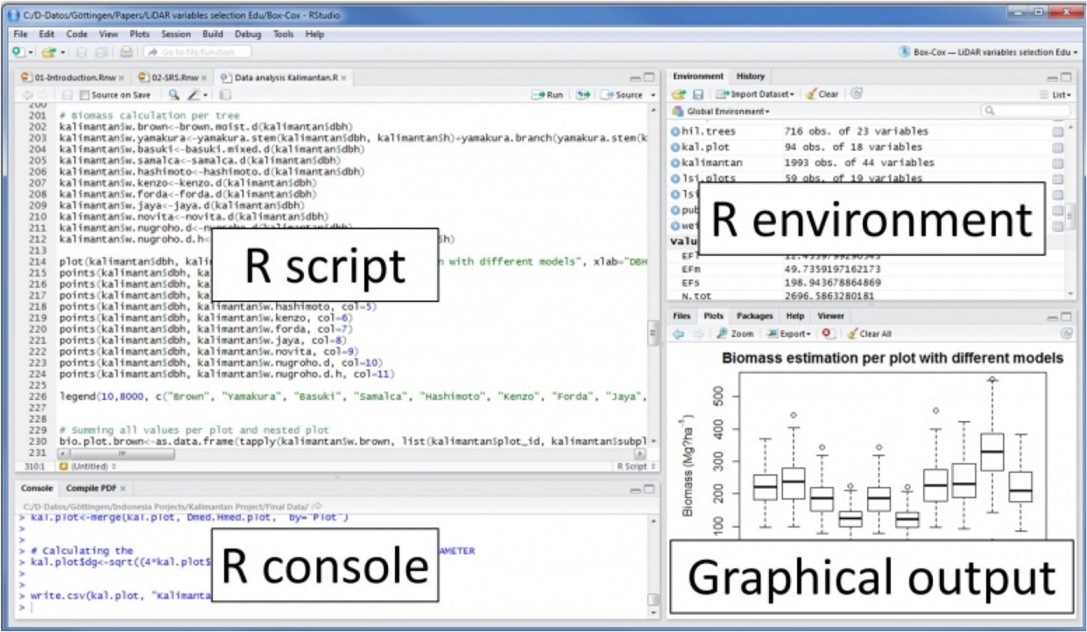
\includegraphics[width=15.1in]{img/RStudioGUI01} 

}

\caption{List of all variables and the description of each variable}\label{fig:unnamed-chunk-1}
\end{figure}

\hypertarget{console}{%
\paragraph{Console}\label{console}}

We can type commands directly into the console, or write in a text file,
and then send the command to the console. It is convenient to use the
console if your task involves on one line of code. Otherwise, we should
always use an editor to write code and then run the code in the Console.

\hypertarget{source-editor}{%
\paragraph{Source Editor}\label{source-editor}}

Generally we will want to write programs longer than a few lines. The
Source Editor can help you open, edit and execute these programs.

\hypertarget{environment-window}{%
\paragraph{Environment Window}\label{environment-window}}

The Environment window shows the objects (i.e., dataframes, arrays,
values and functions) in the environment (workspace). We can see the
descriptive information such as types as dimension of the objects in
your environment. We also choose data source from the environment to
view in the source window like a spreadsheet.

\hypertarget{system-and-graphic-files}{%
\paragraph{System and Graphic files}\label{system-and-graphic-files}}

The Files tab has a navigable file manager, just like the file system on
your operating system. The Plot tab is where graphics you create will
appear. The Packages tab shows you the packages that are installed and
those that can be installed (more on this just now). The Help tab allows
you to search the R documentation for help and is where the help appears
when you ask for it from the Console.

\hypertarget{r-markdown}{%
\subsubsection{R Markdown}\label{r-markdown}}

An R Markdown document is a text based file format that allows you to
include both descriptive text, code blocks and code output. It can be
converted to other types of files such as PDF, HTML, and WORD that can
include code, plots, outputs generated from the code chunks.

\hypertarget{code-chunk}{%
\paragraph{Code Chunk}\label{code-chunk}}

In R Markdown, we can embed R code in the code chunk defined by symbol
\texttt{\textasciigrave{}\textasciigrave{}\textasciigrave{}\{\}} and
closed by \texttt{\textasciigrave{}\textasciigrave{}\textasciigrave{}}.
The symbol \texttt{} `, also called \textbf{backquote} or
\textbf{backtick},can be found on the top left corner of the standard
keyboard as shown in the following.

\begin{figure}

{\centering 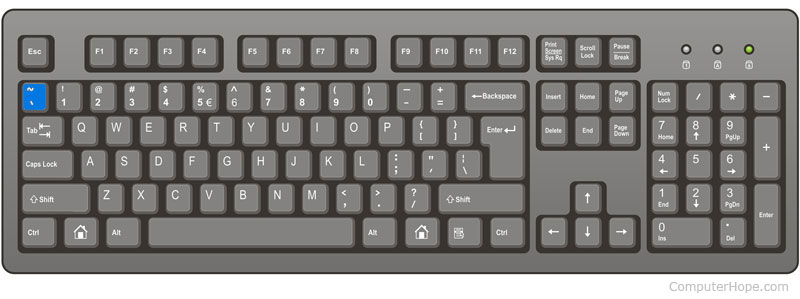
\includegraphics[width=11.11in]{img/Key4CodeChunk} 

}

\caption{The location of backquote on the standard keyboard}\label{fig:unnamed-chunk-2}
\end{figure}

There are two code chunks: executable and non-executable chunks. The
following code chunk is non-executable since is no argument specified in
the \texttt{\{\}}.

\begin{figure}

{\centering 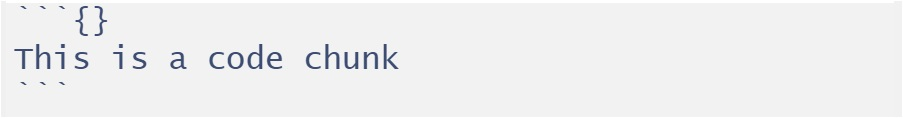
\includegraphics[width=12.14in]{img/Non-executable-code-chunk} 

}

\caption{Non-executable code chunk.}\label{fig:unnamed-chunk-3}
\end{figure}

\begin{verbatim}
This is a code chunk
\end{verbatim}

To write a code chunk that will be executed, we can simply put letter
\texttt{r} inside the curly bracket. If the code the code chunk is
executable, you will the green arrow on the top-right corner of the
chunk.

\begin{figure}

{\centering 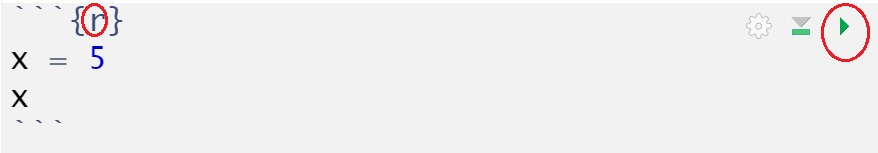
\includegraphics[width=9.39in]{img/Executable-code-chunk} 

}

\caption{Executable code chunk.}\label{fig:unnamed-chunk-4}
\end{figure}

We can define R objects with and without any outputs. In the above R
code chunk, we define an R object under name \texttt{x} and assign value
5 to \texttt{x} (the fist line of the code). We also request an output
that prints the value of \texttt{x}. The above executable code chunk
give output \texttt{{[}1{]}\ 5} in the Markdown document. The same
output in the knit output files is in a box with a transparent
background in the form \texttt{\#\#\ {[}1{]}\ 5}.

\begin{Shaded}
\begin{Highlighting}[]
\NormalTok{x }\OtherTok{=} \DecValTok{5}
\NormalTok{x}
\end{Highlighting}
\end{Shaded}

\begin{verbatim}
## [1] 5
\end{verbatim}

We can also use argument in the code chunk to control the output. For
example, the following code chunk will be evaluate when kitting to other
format of files. But we can still click the green arrow inside the code
chunk to evaluate the code.

\begin{figure}

{\centering 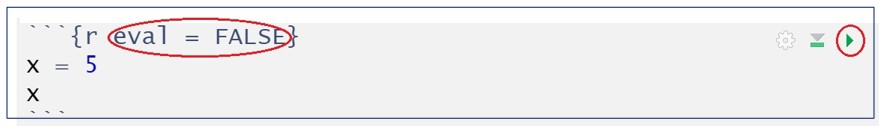
\includegraphics[width=12.21in]{img/Executable-code-chunk-argument} 

}

\caption{Executable code chunk with control options.}\label{fig:unnamed-chunk-6}
\end{figure}

\begin{Shaded}
\begin{Highlighting}[]
\NormalTok{x }\OtherTok{=} \DecValTok{5}
\NormalTok{x}
\end{Highlighting}
\end{Shaded}

\hypertarget{graphics-generated-from-r-code-chunks}{%
\paragraph{Graphics Generated from R Code
Chunks}\label{graphics-generated-from-r-code-chunks}}

In the previous sub-setions, we include images from external image
files. In fact, can use R function to generate graphics (other than
interacting with plots, etc.) in the markdown file \& knit. For
instance, we can generate following image from R and include in the
Markdown document and in the knitter output files.

\begin{Shaded}
\begin{Highlighting}[]
\FunctionTok{library}\NormalTok{(phytools)}
\FunctionTok{data}\NormalTok{(anoletree)}
\FunctionTok{plotTree}\NormalTok{(}\FunctionTok{as.phylo}\NormalTok{(anoletree), }\AttributeTok{type=}\StringTok{"fan"}\NormalTok{, }\AttributeTok{lwd=}\DecValTok{1}\NormalTok{, }\AttributeTok{fsize=}\FloatTok{0.7}\NormalTok{)}
\end{Highlighting}
\end{Shaded}

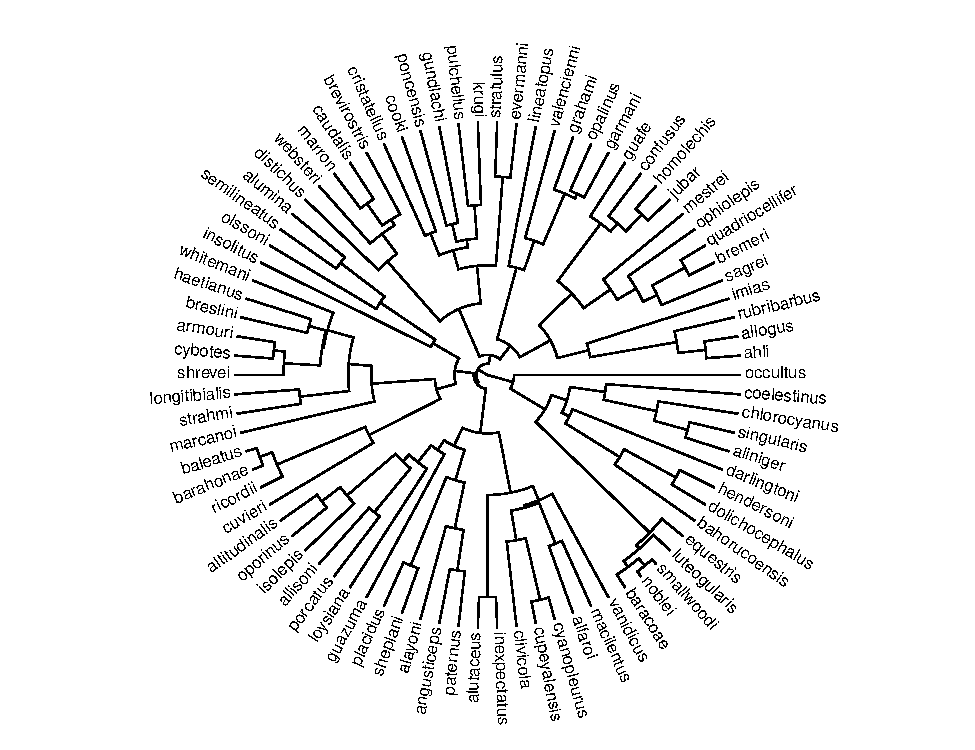
\includegraphics{w01-IntroR-RStudio-Markdown_files/figure-latex/unnamed-chunk-8-1.pdf}

\end{document}
